%%%%%%%%%%%%%%%%%%%%%%%%%%%%%%%%%%%%%%%%%
% Journal Article
% LaTeX Template
% Version 1.3 (9/9/13)
%
% This template has been downloaded from:
% http://www.LaTeXTemplates.com
%
% Original author:
% Frits Wenneker (http://www.howtotex.com)
%
% License:
% CC BY-NC-SA 3.0 (http://creativecommons.org/licenses/by-nc-sa/3.0/)
%
%%%%%%%%%%%%%%%%%%%%%%%%%%%%%%%%%%%%%%%%%

%----------------------------------------------------------------------------------------
%	PACKAGES AND OTHER DOCUMENT CONFIGURATIONS
%----------------------------------------------------------------------------------------

\documentclass[oneside]{article}

\usepackage{lipsum} % Package to generate dummy text throughout this template
\usepackage{amsmath}
\usepackage[sc]{mathpazo} % Use the Palatino font
\usepackage[T1]{fontenc} % Use 8-bit encoding that has 256 glyphs
\linespread{1.05} % Line spacing - Palatino needs more space between lines
\usepackage{microtype} % Slightly tweak font spacing for aesthetics
\usepackage{amsmath}

\usepackage[hmarginratio=1:1,top=32mm,columnsep=20pt]{geometry} % Document margins
\usepackage{multicol} % Used for the two-column layout of the document
\usepackage[hang, small,labelfont=bf,up,textfont=it,up]{caption} % Custom captions under/above floats in tables or figures
\usepackage{booktabs} % Horizontal rules in tables
\usepackage{float} % Required for tables and figures in the multi-column environment - they need to be placed in specific locations with the [H] (e.g. \begin{table}[H])
\usepackage{hyperref} % For hyperlinks in the PDF
\restylefloat{figure}
\usepackage{graphicx}
\usepackage{array}
\newcolumntype{C}[1]{>{\centering\arraybackslash}p{#1}}

\usepackage{lettrine} % The lettrine is the first enlarged letter at the beginning of the text
\usepackage{paralist} % Used for the compactitem environment which makes bullet points with less space between them

\usepackage{abstract} % Allows abstract customization
\renewcommand{\abstractnamefont}{\normalfont\bfseries} % Set the "Abstract" text to bold
%\renewcommand{\abstracttextfont}{\normalfont\small\itshape} % Set the abstract itself to small italic text

\usepackage{titlesec} % Allows customization of titles
%\renewcommand\thesection{\Roman{section}} % Roman numerals for the sections
%\renewcommand\thesubsection{\Roman{subsection}} % Roman numerals for subsections
%\titleformat{\section}[block]{\large\scshape\centering}{\thesection.}{1em}{} % Change the look of the section titles
\titleformat{\subsection}[block]{\large}{\thesubsection.}{1em}{} % Change the look of the section titles

\usepackage{fancyhdr} % Headers and footers
\pagestyle{fancy} % All pages have headers and footers
\fancyhead{} % Blank out the default header
\fancyfoot{} % Blank out the default footer
%\fancyhead[C]{Hall C Collaboration $\bullet$ \today} % Custom header text
\fancyhead[C]{\today} % Custom header text
\fancyfoot[RO,LE]{\thepage} % Custom footer text
\usepackage{authblk}

%----------------------------------------------------------------------------------------
%	TITLE SECTION
%----------------------------------------------------------------------------------------

\title{\vspace{-15mm}\fontsize{20pt}{10pt}\selectfont\textbf{A new method to study the EMC Effect using the $F_2^{n}$ structure function}} % Article title

\author[1]{H. Szumila-Vance}
\author[2]{I. Cloet}
\author[1]{C. Keppel}
\author[3]{N. Kalentarians}
\affil[1]{Thomas Jefferson National Accelerator Facility, Newport News, VA}
\affil[2]{Argonne National Laboratory, Argonne, IL}
\affil[3]{Virginia Union University, Richmond, VA}
\renewcommand\Authands{ , }



%\author{
%\large
%\textsc{Holly Szumila-Vance}\thanks{}\\[2mm] % Your name
%\normalsize Jefferson Lab \\ % Your institution
%\normalsize \href{mailto:hszumila@jlab.org}{hszumila@jlab.org} % Your email address
%\vspace{-5mm}
%}
\date{}

%----------------------------------------------------------------------------------------

\begin{document}

\maketitle % Insert title

\thispagestyle{fancy} % All pages have headers and footers

%----------------------------------------------------------------------------------------
%	ABSTRACT
%----------------------------------------------------------------------------------------

\begin{abstract}
The EMC effect is the go-to observable in the deep inelastic scattering regime that explains how nucleons in bound nuclei are modified compared to bound nucleons in deuterium.  The free neutron structure function has recently been extracted in a systematic study of the world data and is available as part of the Jefferson Lab-CTEQ Collaboration. Here we introduce a new method to study the EMC Effect in nuclei by re-examining data from the SLAC E139 experiment and determining the magnitude of the EMC Effect using the free neutron and free proton structure functions in the denominator. From the extraction of the free neutron from world data, it is possible to examine the nuclear effects in deuterium and their contribution to our interpretation of the EMC Effect.

\end{abstract}
%\newpage
%\tableofcontents
%\newpage
 %\listoffigures
% \newpage
%\listoftables
%\newpage
%----------------------------------------------------------------------------------------
%	ARTICLE CONTENTS
%----------------------------------------------------------------------------------------


\section{Introduction}

We chose to use the SLAC E139 data set because it is the most complete published list of cross sections available. From the initial cross sections given, we converted the absolute cross section to the structure function by using the kinematics and R1990 fitting. 

  
\section{Theory predictions using nuclear matter}

Ian can write something here.
  
\section{$F_2^n$ extraction and the CJ15 fit}

We need to point to CJ and how the world data was extracted. 

 \begin{figure}
\begin{minipage}{0.5\textwidth}
 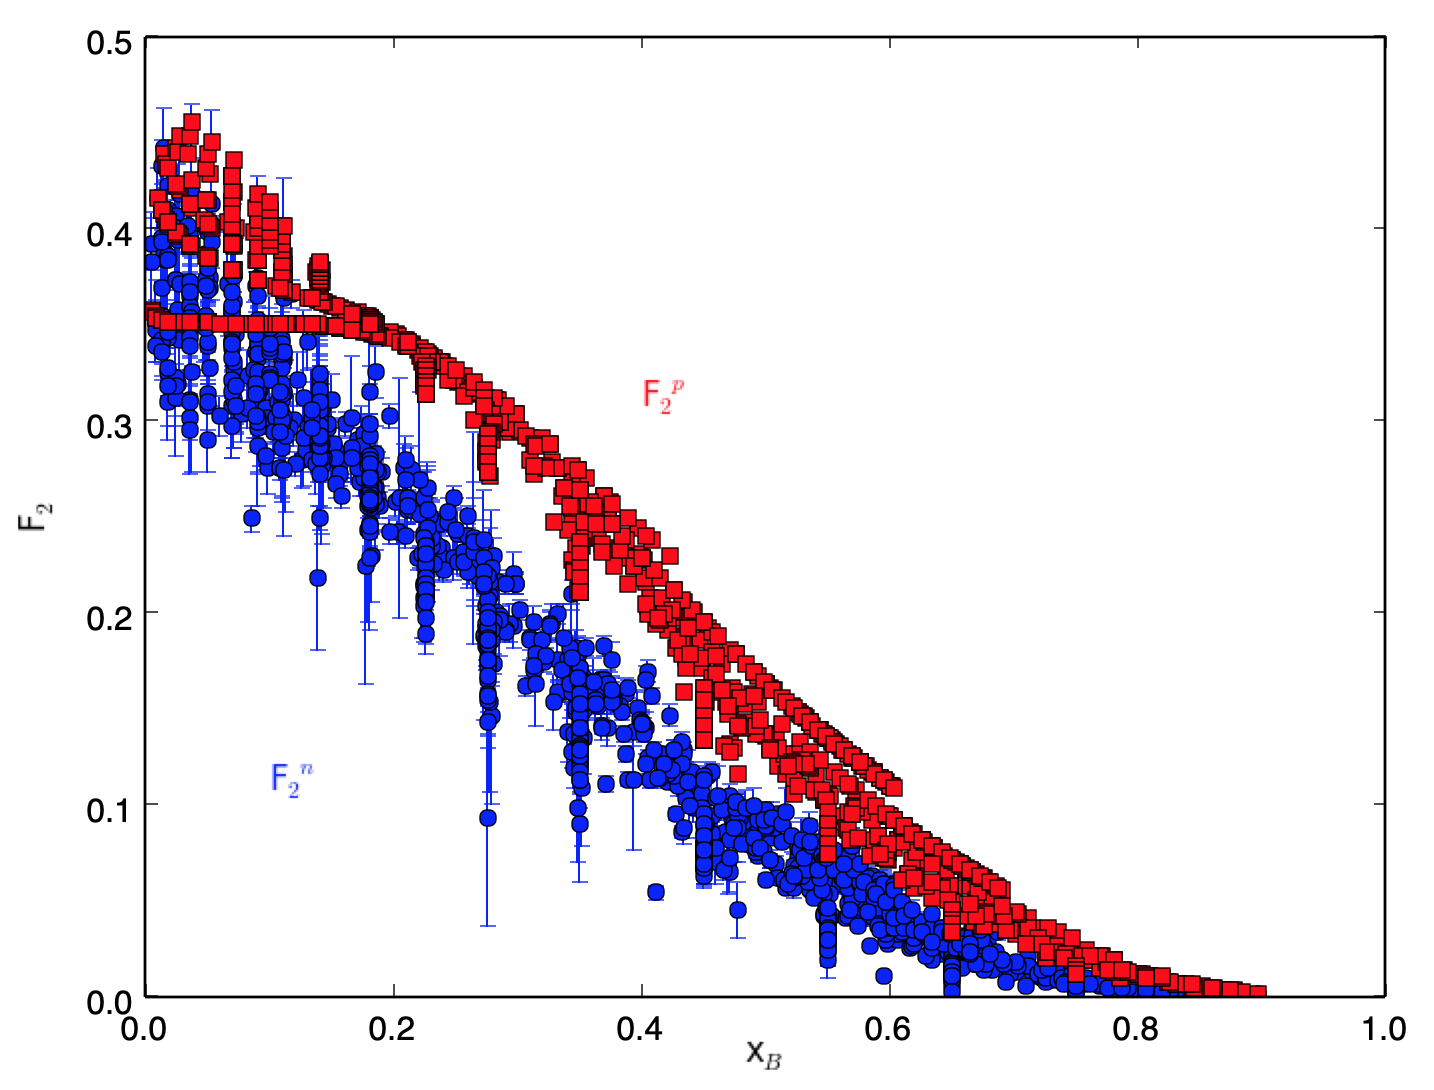
\includegraphics[width=\textwidth]{plots/f2np_plot.png}
\end{minipage}\hfill\begin{minipage}{0.5\textwidth}
 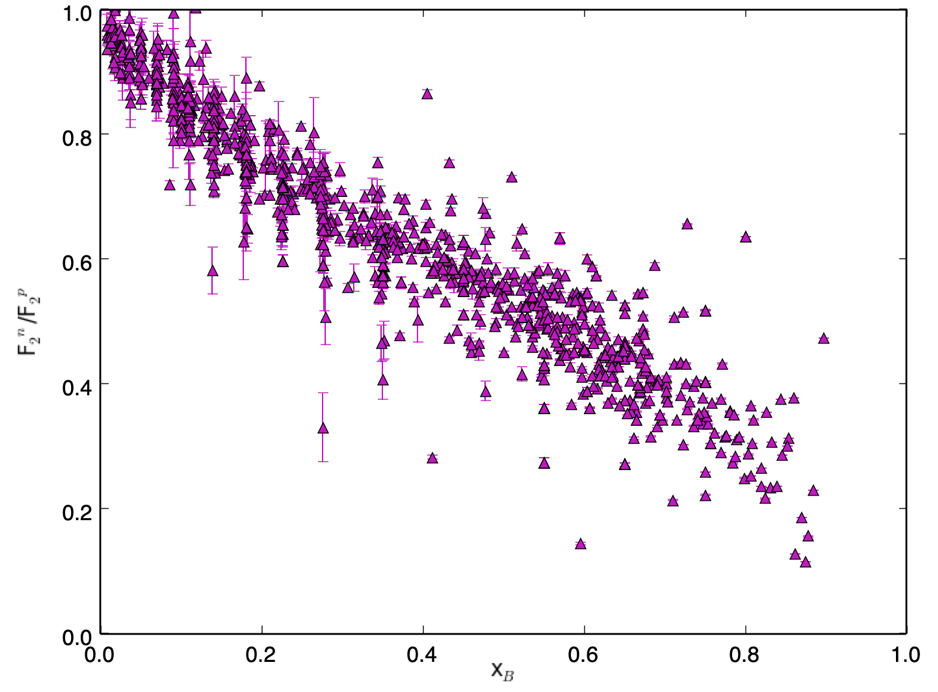
\includegraphics[width=\textwidth]{plots/f2npratio_plot.png}
 \end{minipage}
  \caption[$F_2^{n,p}$ characteristics]{Left: The extracted $F_2^n$ from the world DIS data is shown in blue, and the $F_2^p$ from the NMC global fit is shown in red for the same corresponding $x_B$ and $Q^2$. Right: The ratio of the $F_2^n/F_2^p$ from the left is shown as a function of $x_B$.}
  \label{fig:F2np_general}
\end{figure} 
 
\subsection{$Q^2$ dependence}

\begin{figure}
\begin{minipage}{0.5\textwidth}
 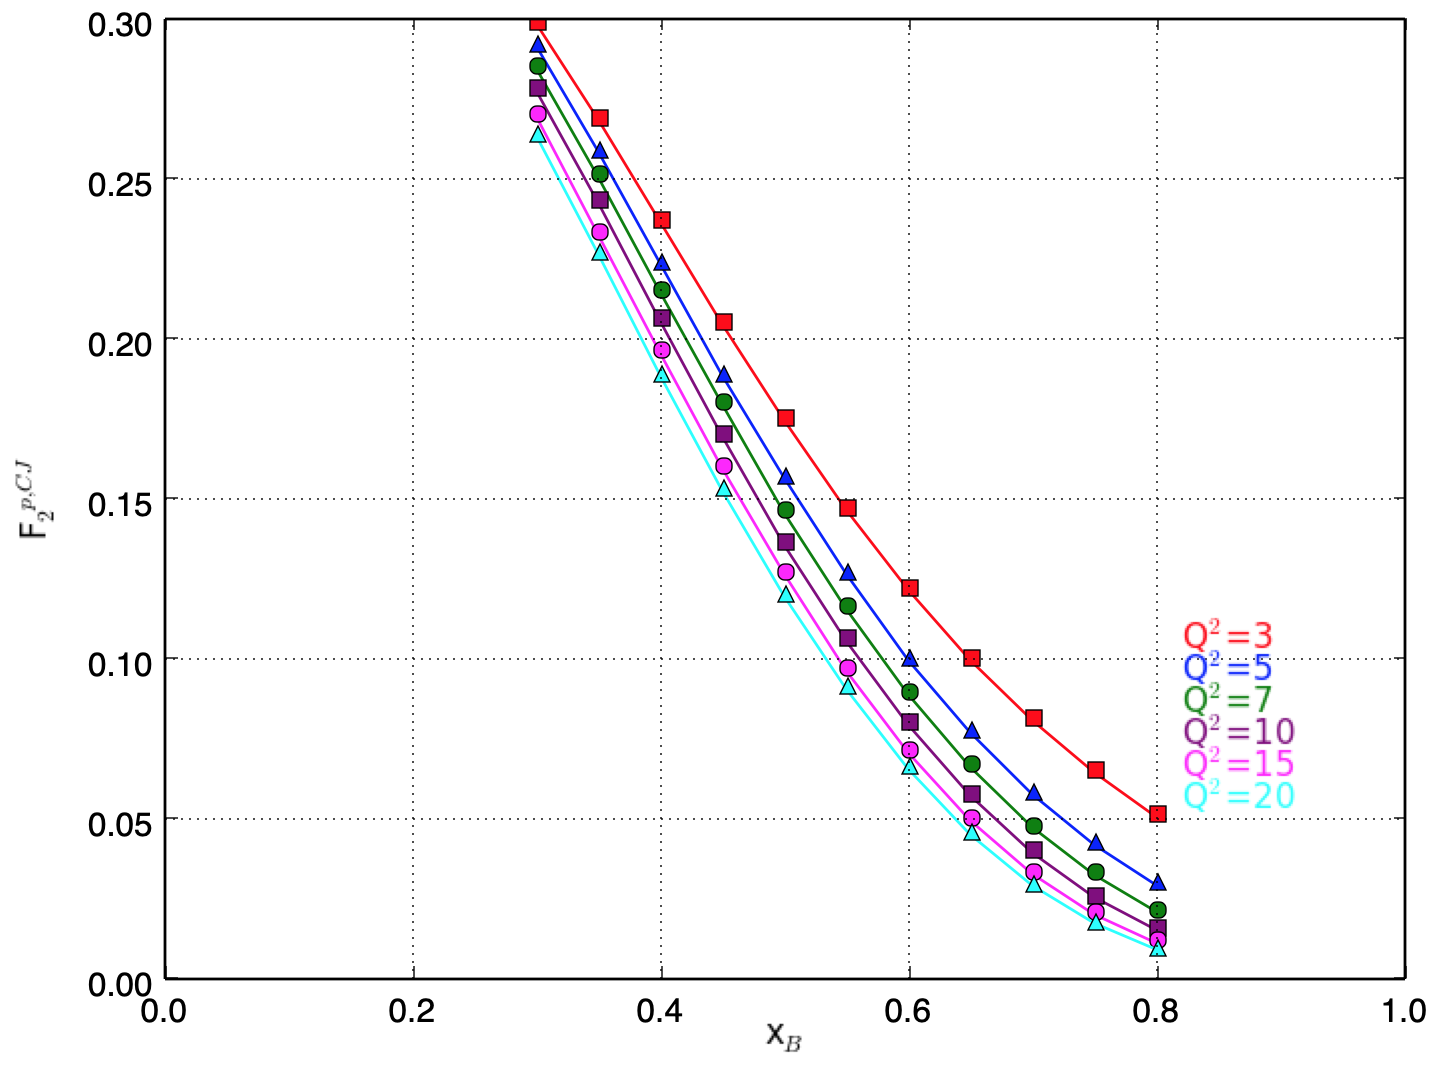
\includegraphics[width=\textwidth]{plots/p_CJ.png}
\end{minipage}\hfill\begin{minipage}{0.5\textwidth}
 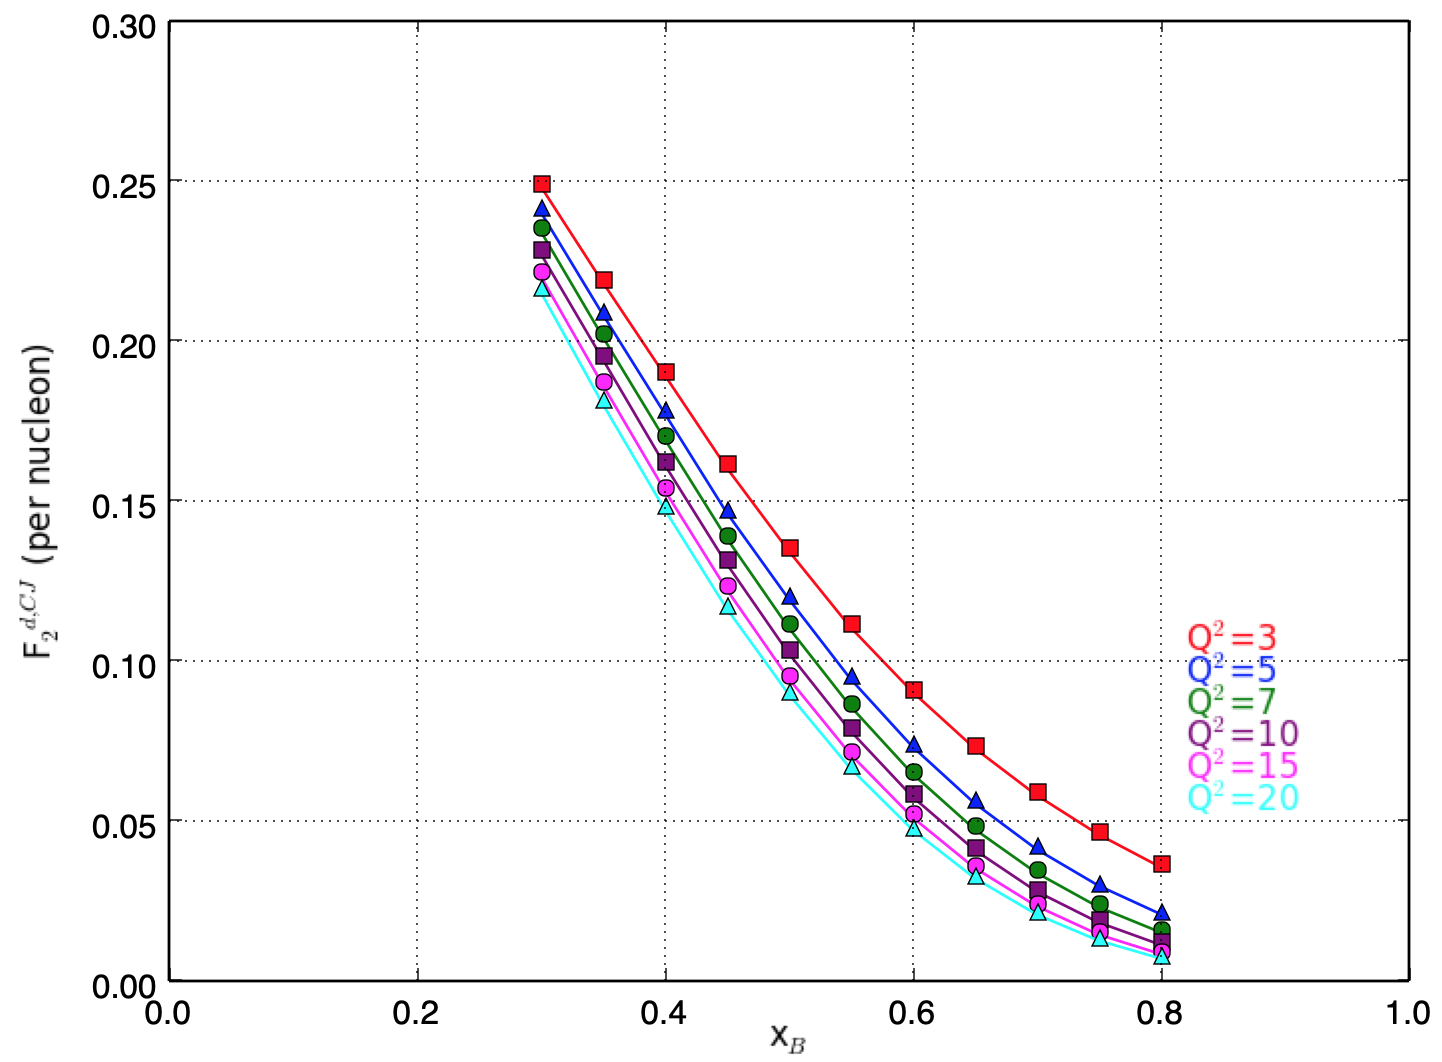
\includegraphics[width=\textwidth]{plots/d_CJ.png}
 \end{minipage}
  \caption[Proton and deuteron from CJ15]{Left: The proton structure function from the CJ15 fit is shown as a function of $x_B$ for various fixed $Q^2$. Right: The deuteron structure function from the CJ15 fit is shown as a function of $x_B$ for various fixed $Q^2$.}
  \label{fig:pd_CJ15}
\end{figure} 
 
\begin{figure}[H]
  \centering
      	  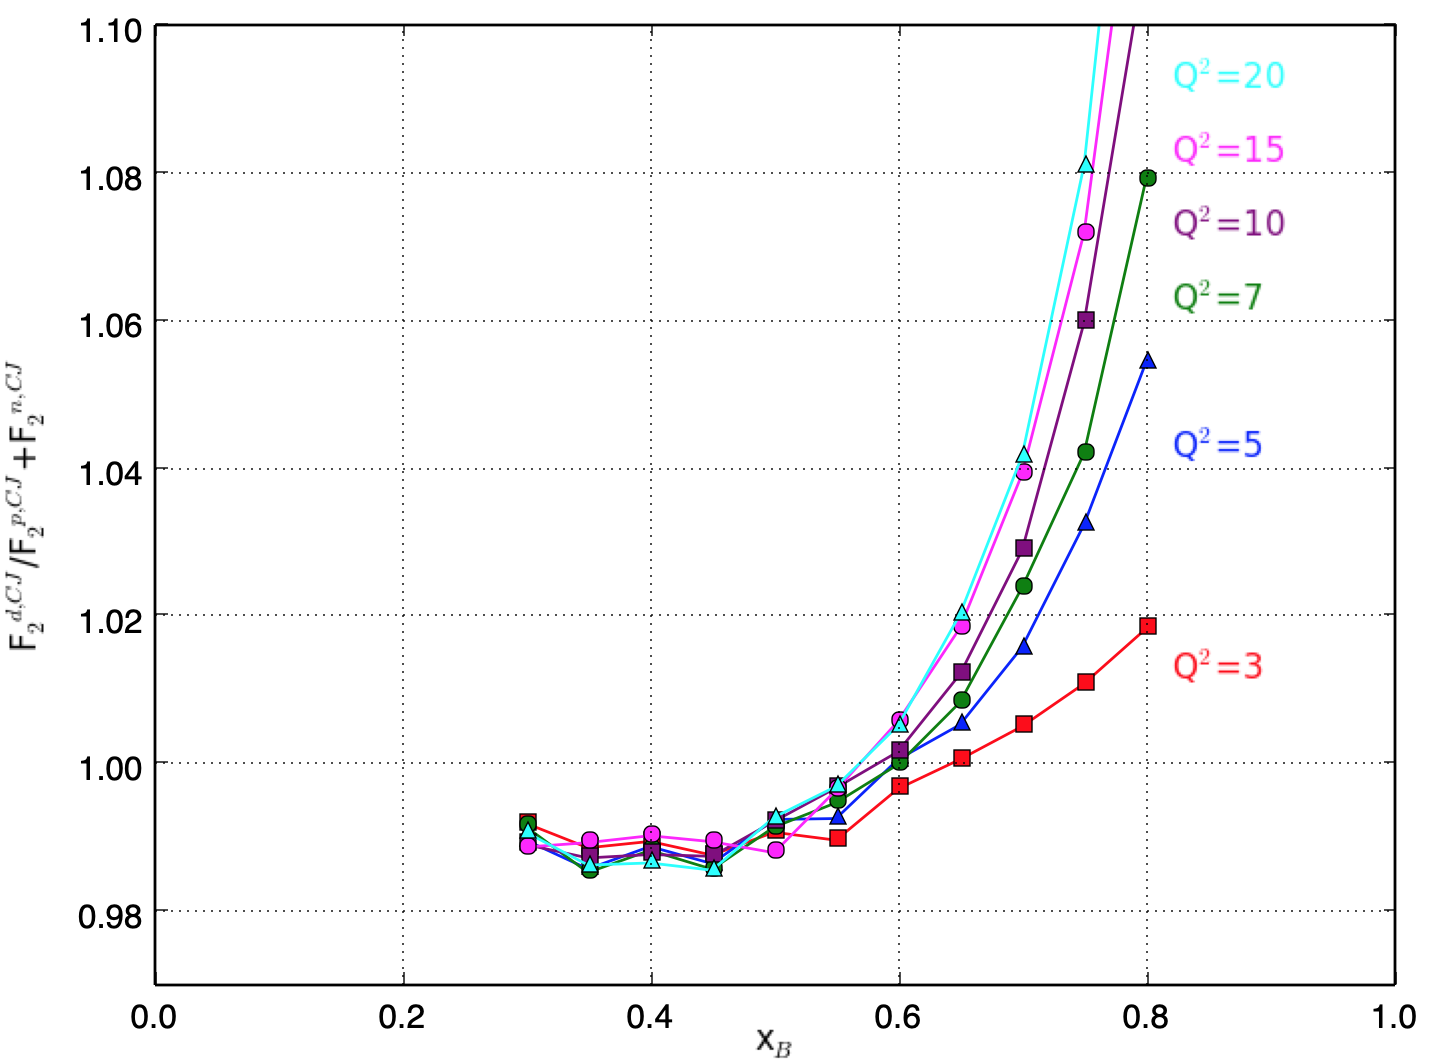
\includegraphics[width=0.5\textwidth]{plots/dpn_allCJ.png}
 	 \caption[Deuteron structure function from CJ15]{The deuteron structure function divided by the sum of the free proton and free neutron structure functions from the CJ15 fit is shown for various $Q^2$. This ratio roughly shows the magnitude of the nuclear effects in the deuteron. The $Q^2$ dependence shows significant spread above $x_B=0.6$ where the ratio begins to increase.}
  \label{fig:dpn_cj}
 \end{figure} 
 
  \begin{figure}
\begin{minipage}{0.5\textwidth}
 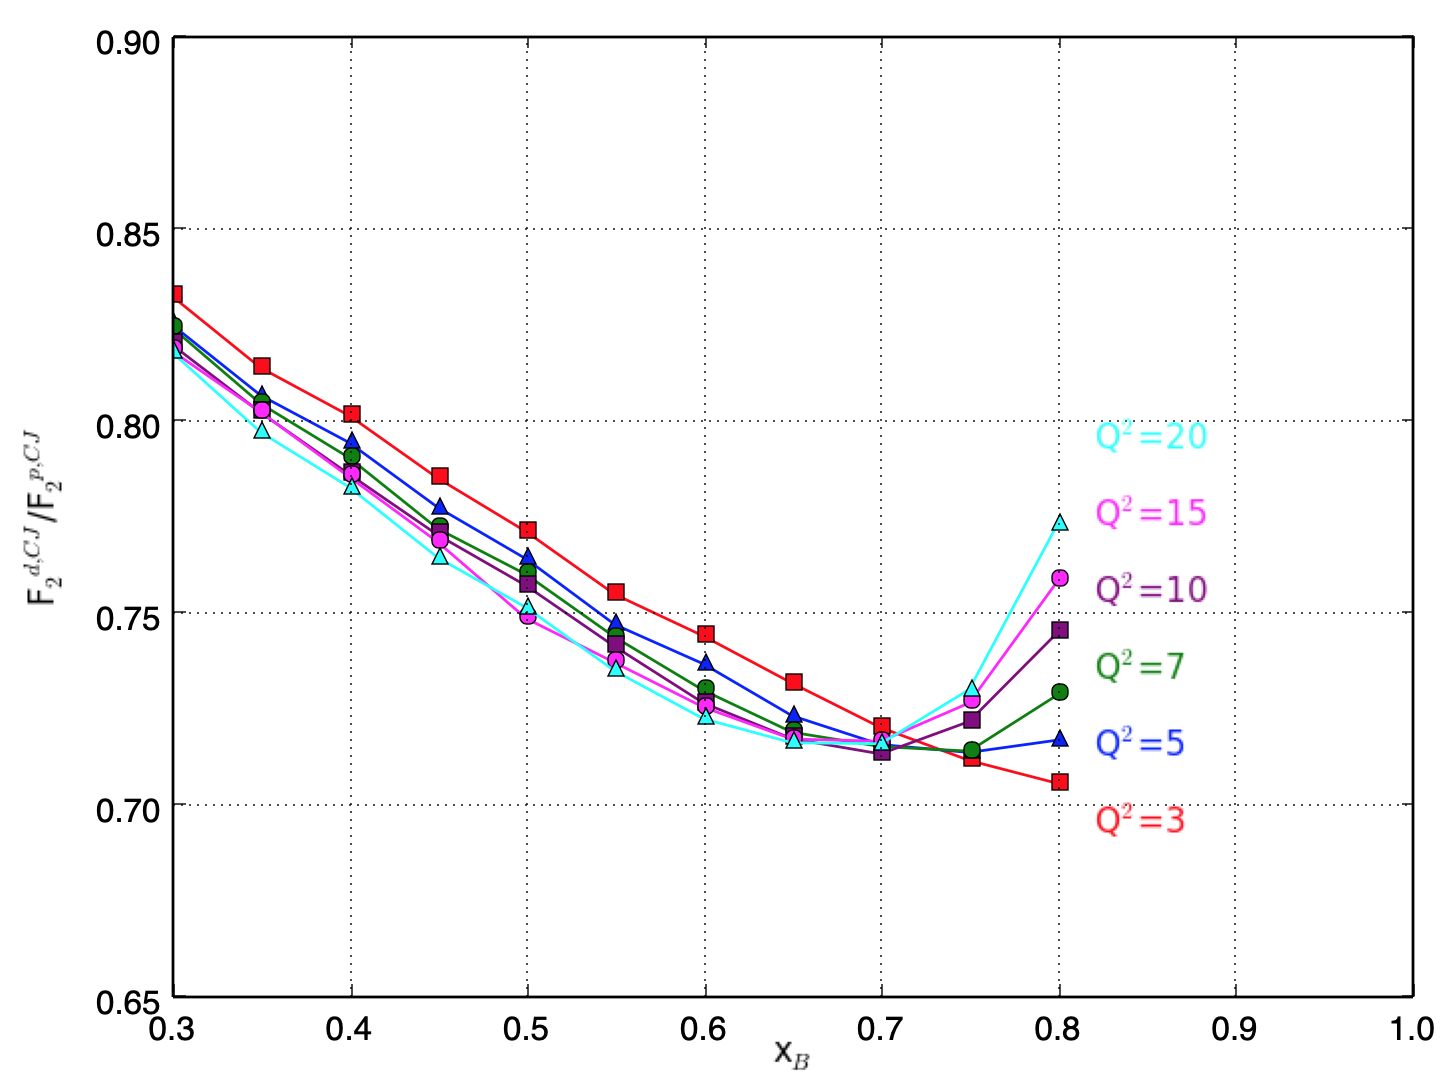
\includegraphics[width=\textwidth]{plots/dpratio_CJ.png}
\end{minipage}\hfill\begin{minipage}{0.5\textwidth}
 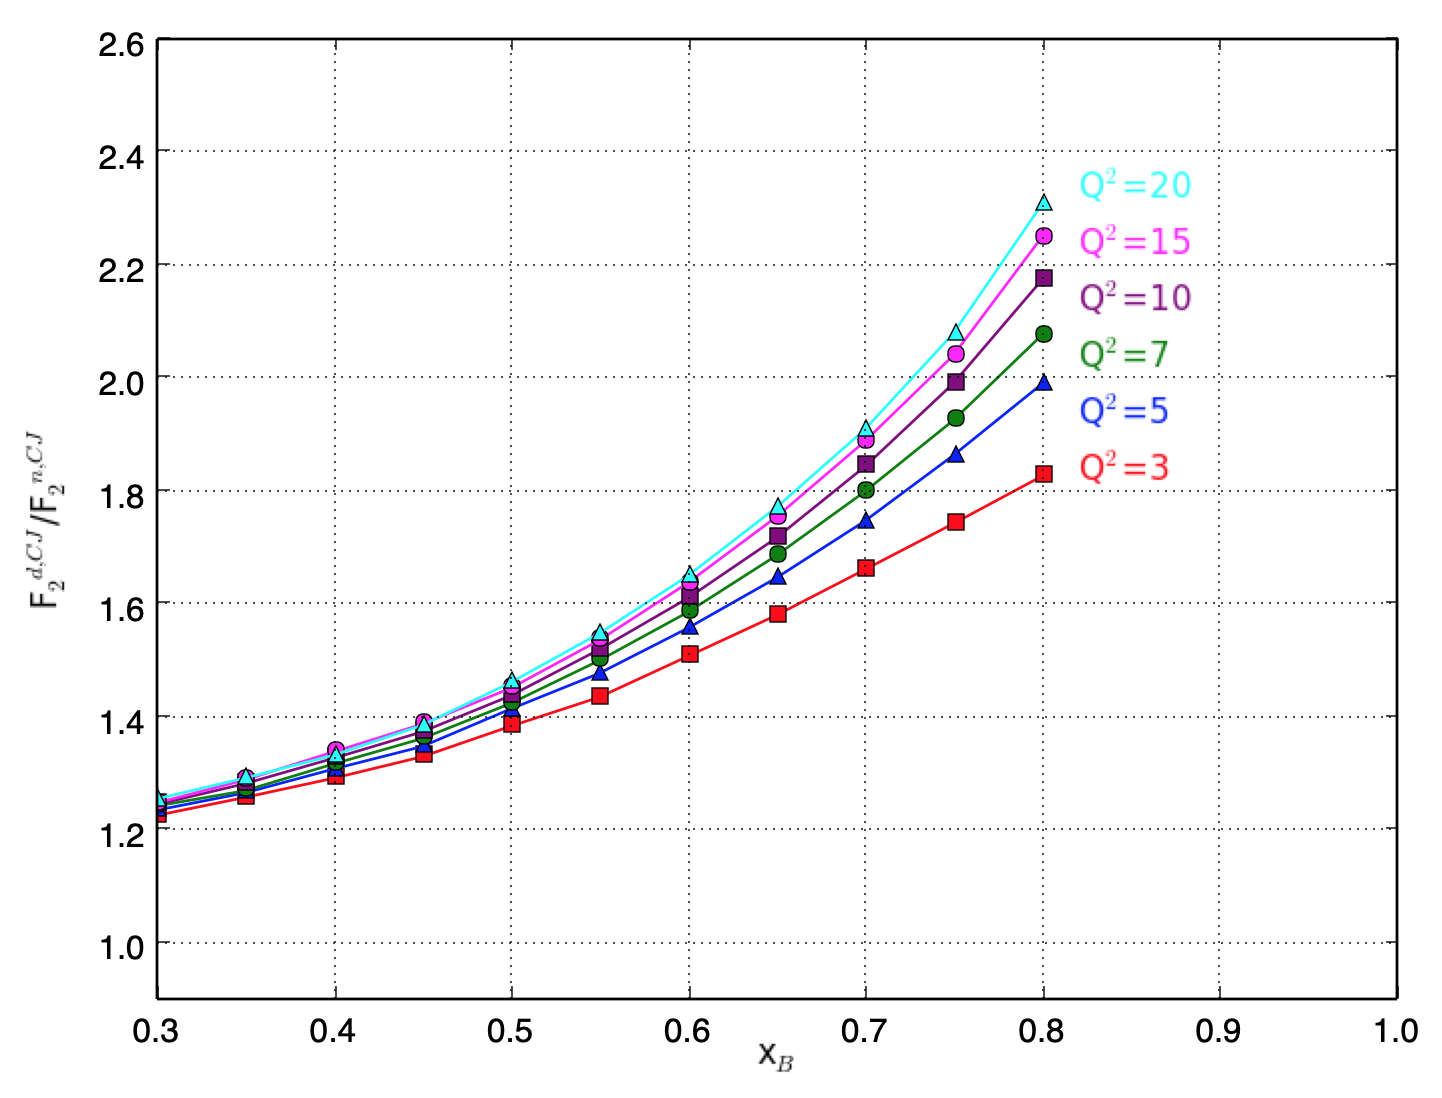
\includegraphics[width=\textwidth]{plots/dnratio_CJ.png}
 \end{minipage}
  \caption[Deuteron ratios from CJ15]{Left: The deuterium structure function from the CJ15 fit is shown as a ratio to the proton structure function from CJ15 for various $Q^2$. Right: The deuterium structure function from the CJ15 fit is shown as a ratio to the neutron structure function from CJ15 for various $Q^2$.}
  \label{fig:dratio_cj}
\end{figure} 

\section{Structure function extraction from the E139 cross sections}

Discuss the input cross section, conversion to F2A and the iso-scalar correction.

\begin{equation}
F_2 = \dfrac{d^2\sigma}{d\Omega dE'}\dfrac{1+R}{1+\epsilon R}\dfrac{K\nu}{4\pi^2\alpha\Gamma (1+\nu^2/Q^2)}
\label{eq:matrixelements}
\end{equation}

\begin{align}
\epsilon=&(1+2\dfrac{\nu^2+Q^2}{Q^2}tan^2\dfrac{\theta}{2})^{-1}\\
K=&\dfrac{W^2-M^2}{2M}\\
\Gamma=&\dfrac{\alpha KE'}{2\pi^2Q^2E(1-\epsilon)}
\label{eq:matrixeqn}
\end{align}

\begin{equation}
f_{iso}^A = \dfrac{\dfrac{1}{2}(1+F_2^n/F_2^p)}{\dfrac{1}{A}(Z+(A-Z)F_2^n/F_2^p)}
\label{eq:matrixelements}
\end{equation}

\begin{figure}[H]
  \centering
      	  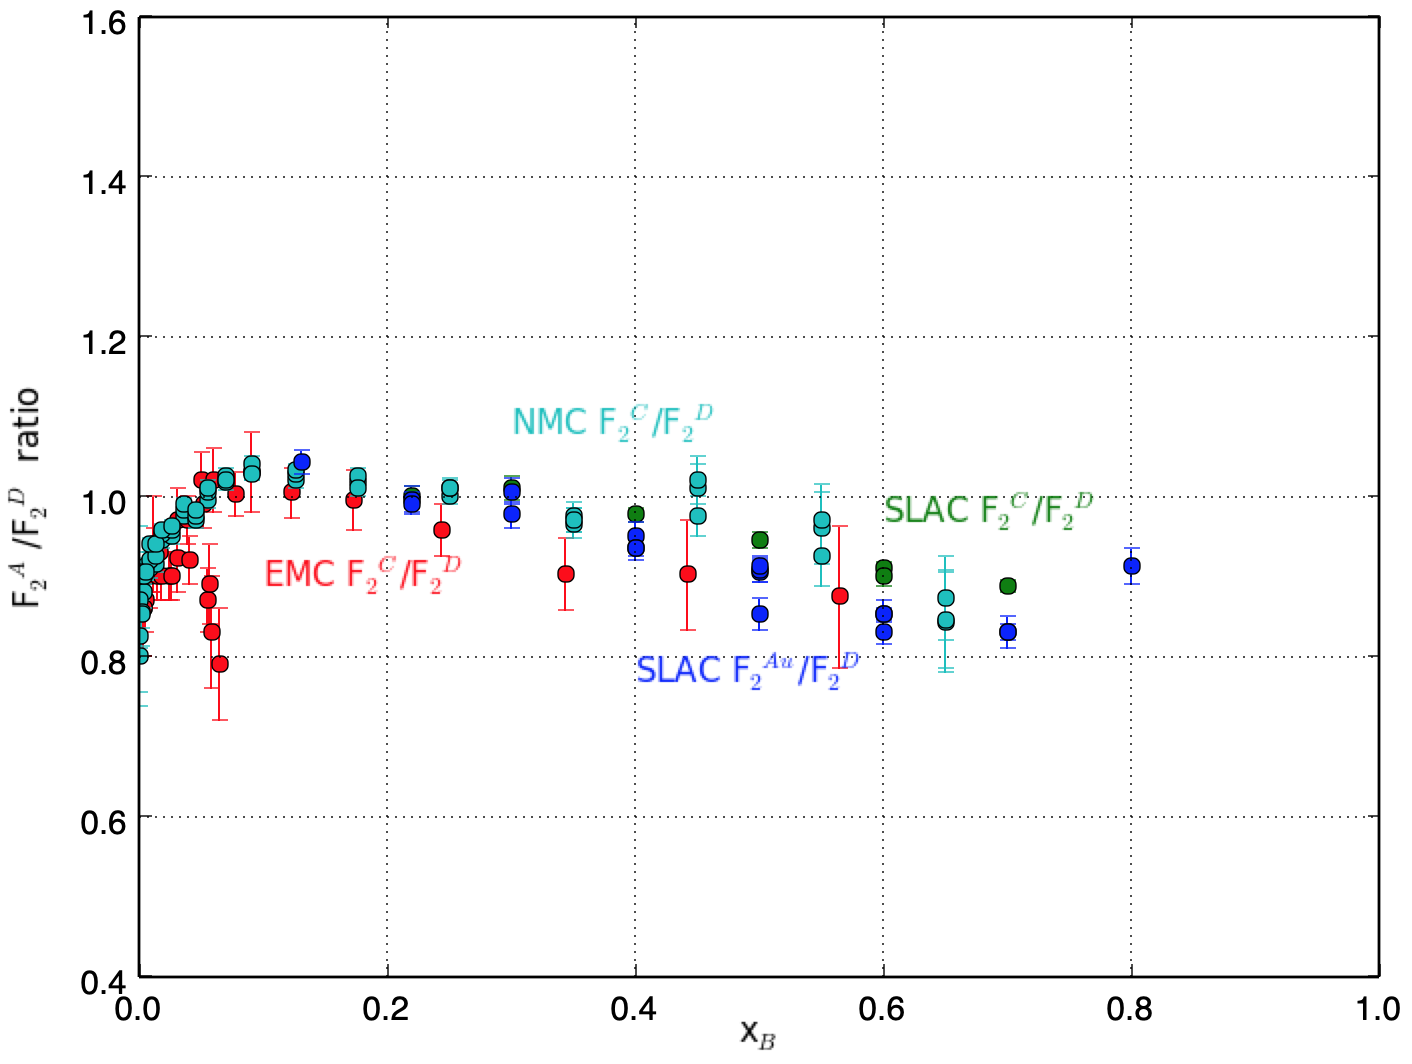
\includegraphics[width=0.5\textwidth]{plots/emc_ratios_data.png}
 	 \caption[EMC ratios for various data]{The published structure function ratios per nucleon for carbon and gold are shown from SLAC, NMC, and the EMC experiments.}
  \label{fig:emc_ratios}
 \end{figure}

\section{General observations}
 
  \begin{figure}
\begin{minipage}{0.5\textwidth}
 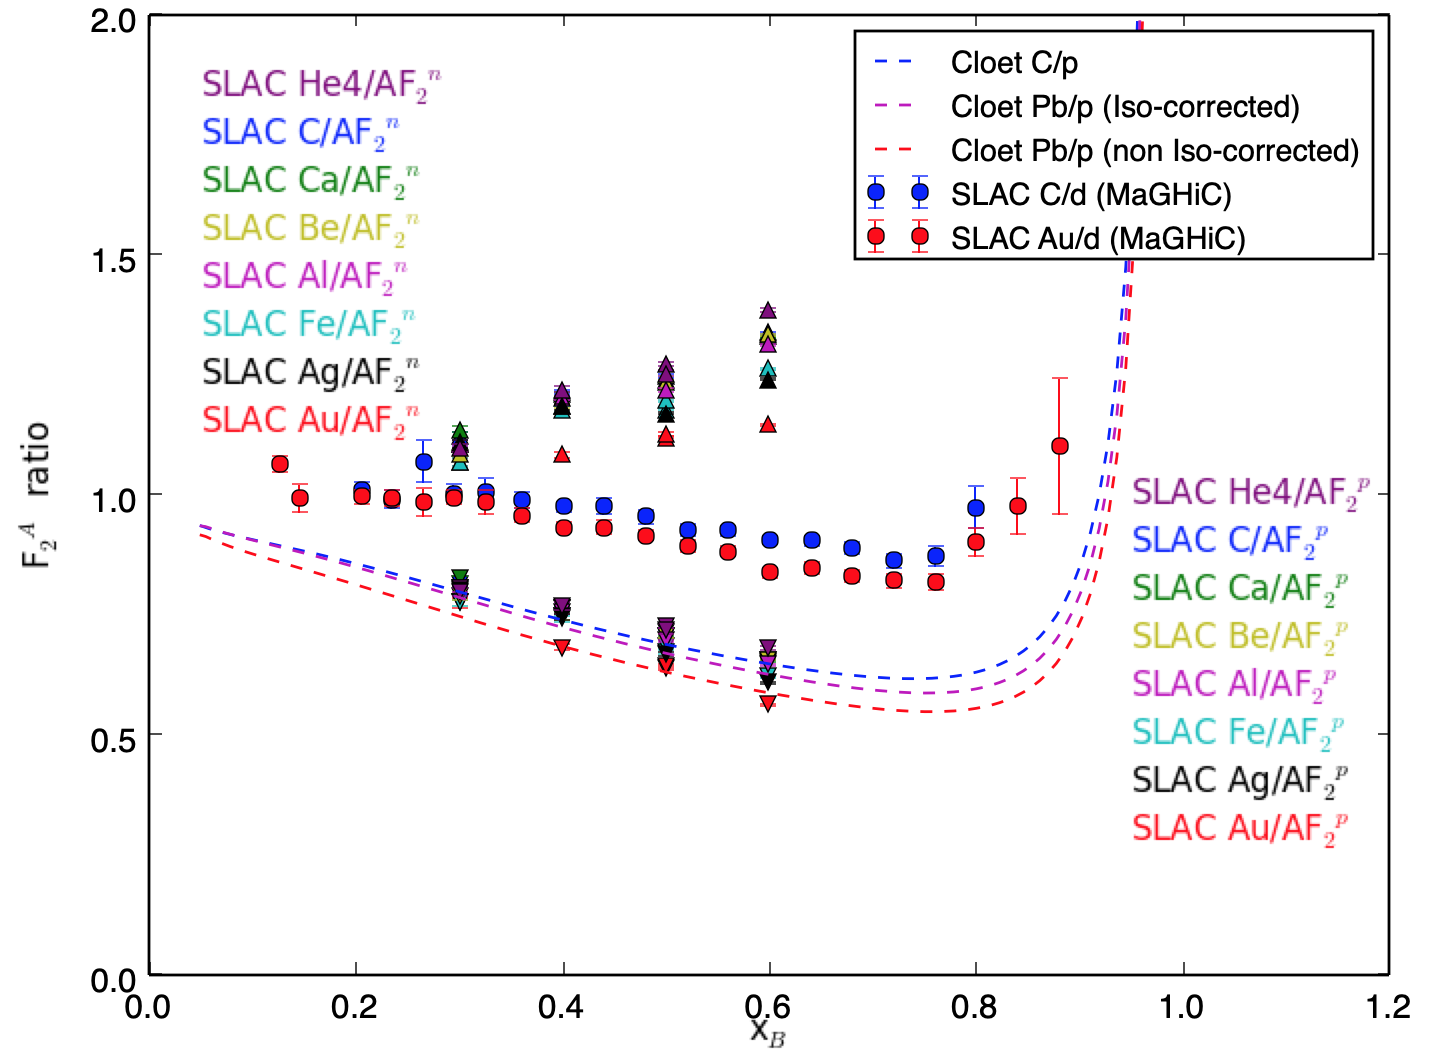
\includegraphics[width=\textwidth]{plots/Anp_data_ratio.png}
\end{minipage}\hfill\begin{minipage}{0.5\textwidth}
 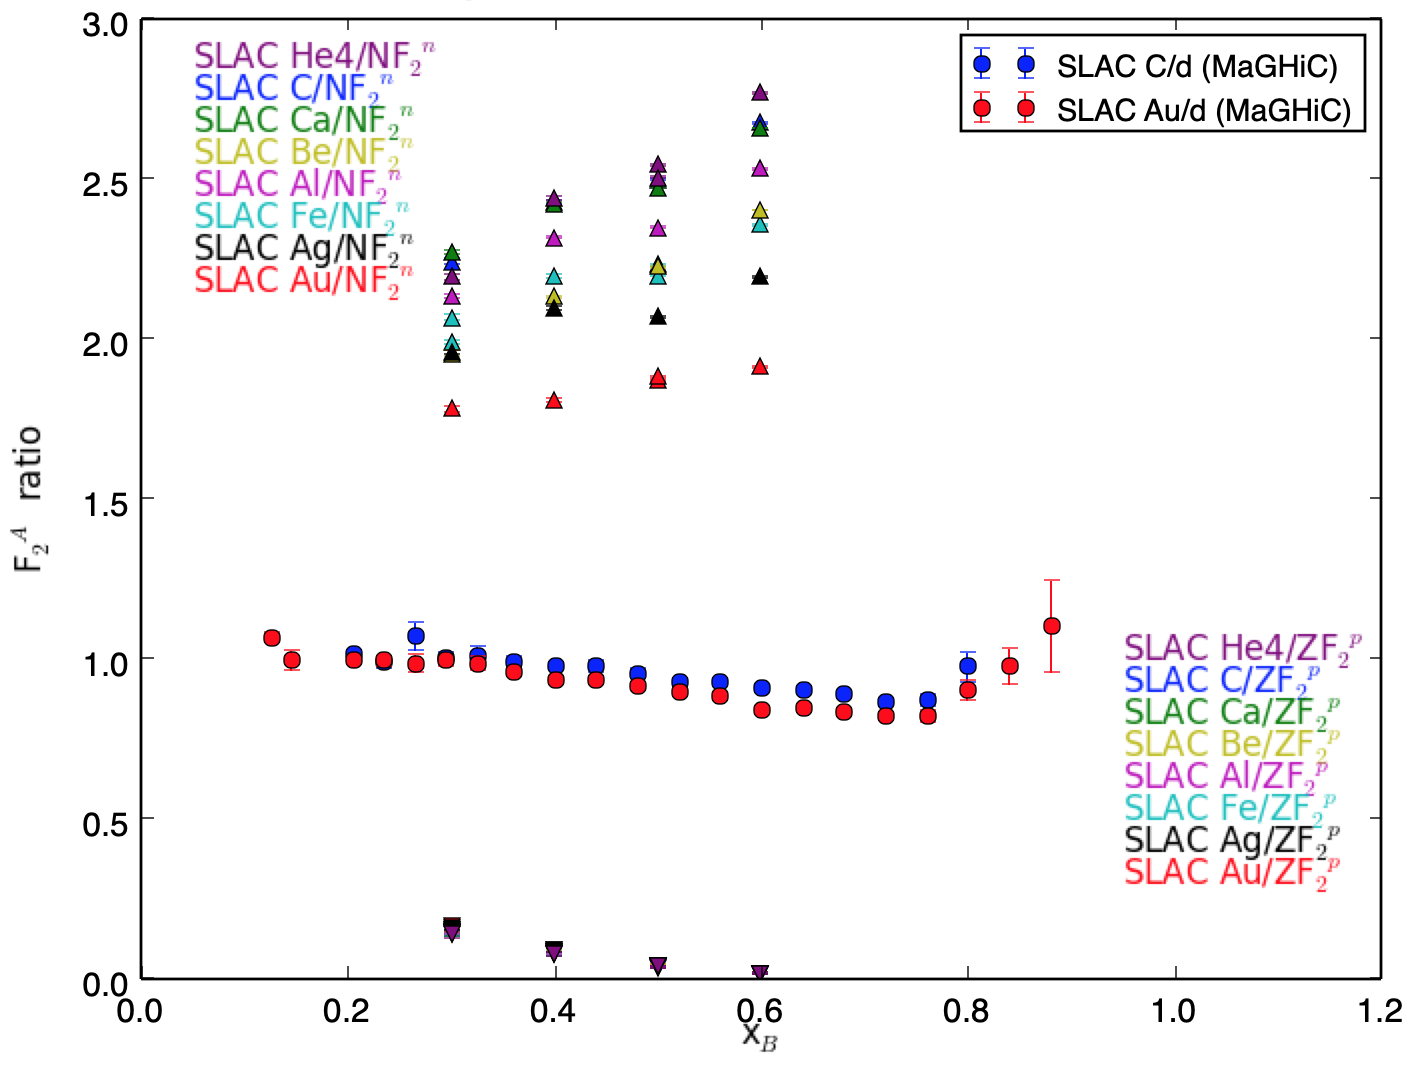
\includegraphics[width=\textwidth]{plots/AZNnp_data_ratio.png}
 \end{minipage}
  \caption[$F_2^A$ ratio to $F_2^n$ and $F_2^p$]{Left: $F_2^A$ calculated from the published SLAC E139 cross sections is taken as a ratio per nucleon to $F_2^n$ and $F_2^p$, separately. The published EMC ratios for carbon and gold~\cite{Malace:2014uea} are shown for reference as $F_2^A/F_2^d$ per nucleon. Theory predictions for the $F_2^A$ structure function per nucleon as a ratio to $F_2^p$ are shown. Right: $F_2^A$ calculated from the published SLAC E139 cross sections is taken as a ratio per neutron or proton and $F_2^n$ and $F_2^p$, separately. The published EMC ratios for carbon and gold~\cite{Malace:2014uea} are shown for reference.}
  \label{fig:data_np_ratio}
\end{figure}  
 
 
\section{Deuterium nuclear effects and heavier nuclei}

\subsection{Deuterium}

\begin{figure}[H]
  \centering
      	  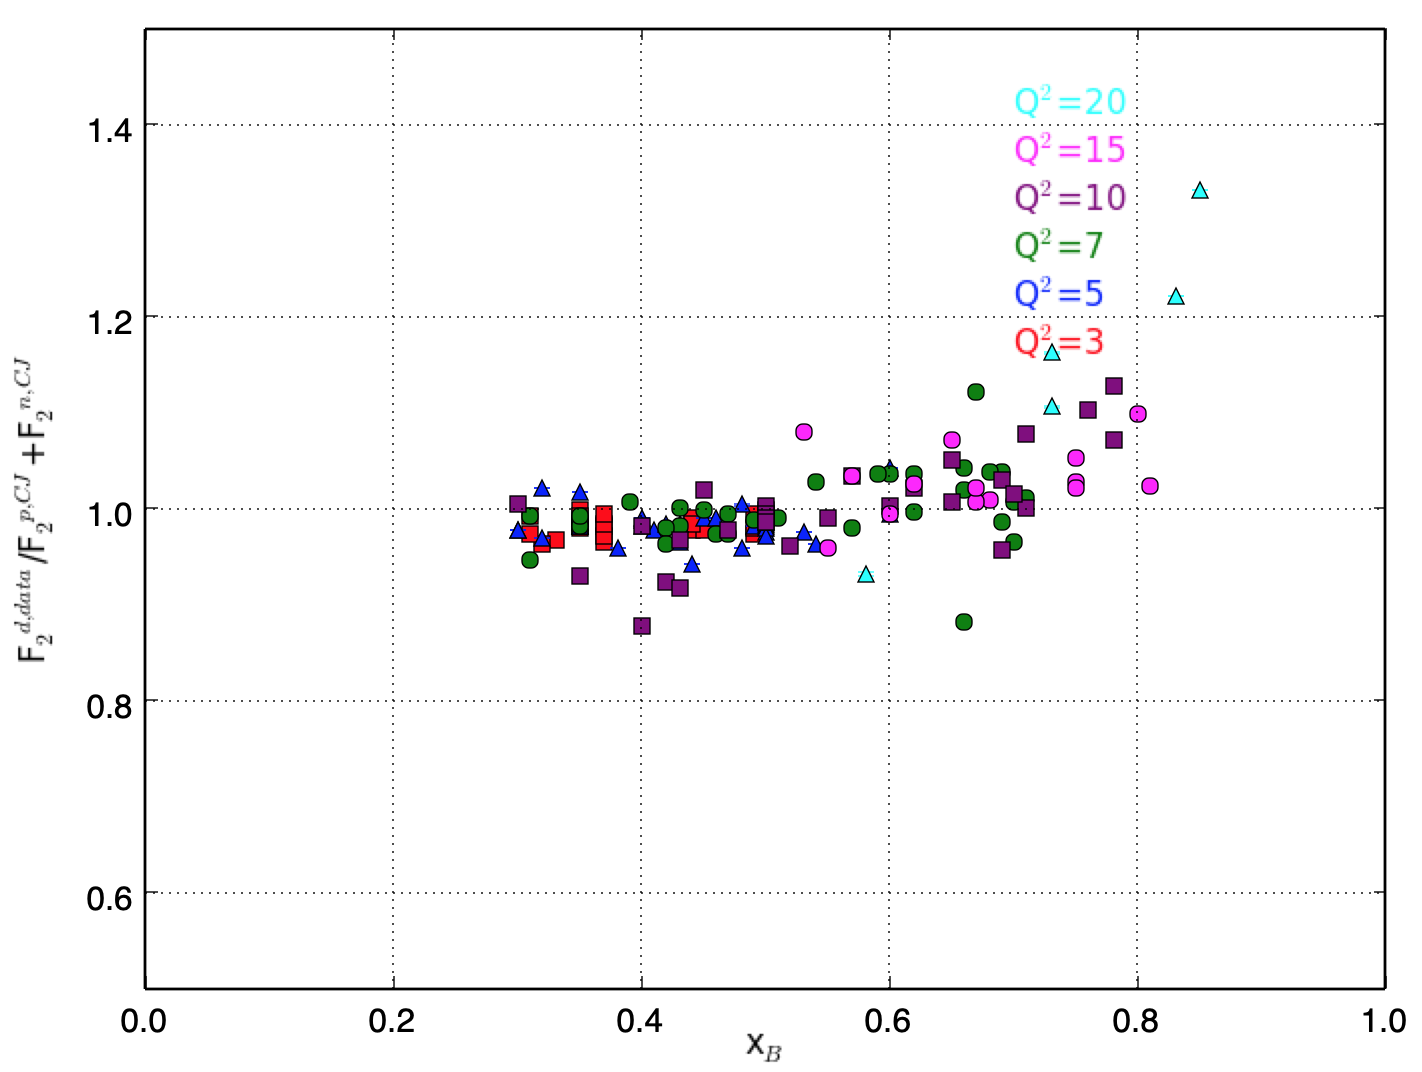
\includegraphics[width=0.5\textwidth]{plots/deuterium_q2.png}
 	 \caption[Deuterium data from SLAC]{The global Whitlow deuterium data from SLAC~\cite{XS_d} is shown divided by the sum of the free proton and free neutron structure functions from the CJ15 fit.}
  \label{fig:d2_q2}
 \end{figure}

plots: include d/n or n/d of Whitlow+BONUS to show Q2 dependency

\subsection{Heavier nuclei}

Include a table of the fit slopes with errors
\begin{table}[htb!]
\caption{\label{SlopeFits} Summary of linear fits to $x_B$.}
\centering
\begin{tabular}{ | C{2.5cm} | C{2cm} | C{2cm} | C{2cm} | C{2cm} | }
 \hline
 \textbf{Nucleus} & \textbf{A/d slope} & \textbf{A/d intercept} & \textbf{A/(n+p) slope} & \textbf{A/(n+p) intercept} \\ 
  \hline
%HB & $6.485E-03$ & $0.003$ & v6 & v6 & 0.983 \\ 
  %\hline
 % Q1 & $7.103E-03$ & $0.004$ & v0-v2, v6 & v0-v2 & 0.983$\times$0.97 \\ 
  %\hline
  % Q2 & $9.436E-03$ & $0.003$ & -- & -- & 0.983$\times$0.96 \\ 
  %\hline
  % Q3 & $9.728E-03$ & $0.004$ & v0-v2 & -- & 0.983$\times$0.97 \\ 
  %\hline
   % dipole & $1.184E-02$ & $3.188e-03$ & v0-v5 & -- & 0.983 \\ 
  \hline
    \end{tabular}
\end{table} 




\section{Conclusions}
n and p have Q2 dependence and deuterium is not so linear. 



\section{Acknowledgments}

The authors would like to thank Shujie Li for constructing the most complete world $F_2^n$ data set to date and Alberto Accardi and Wally Melnitchouk for providing crucial insights and interpretations for this analysis.  

%----------------------------------------------------------------------------------------
%	REFERENCE LIST
%----------------------------------------------------------------------------------------

\begin{thebibliography}{99} 

\bibitem{CJ15Fit} A. Accardi, L. T. Brady, W. Melnitchouk, J. F. Owens and N. Sato, Phys.Rev. D93 (2016) 114017

\bibitem{Gomez:1993ri} 
  J.~Gomez {\it et al.},
  ``Measurement of the A-dependence of deep inelastic electron scattering,''
  Phys.\ Rev.\ D {\bf 49}, 4348 (1994).
  doi:10.1103/PhysRevD.49.4348

\bibitem{Griffioen:2015hxa} 
  K.~A.~Griffioen {\it et al.},
  ``Measurement of the EMC Effect in the Deuteron,''
  Phys.\ Rev.\ C {\bf 92}, no. 1, 015211 (2015)
  doi:10.1103/PhysRevC.92.015211
  [arXiv:1506.00871 [hep-ph]].

\bibitem{Rubin:2011} 
  J.~G.~Rubin, J.~Arrington,
  ``A New Extraction of Neutron Structure Functions from Existing Inclusive DIS Data,''
  doi:	10.1063/1.3631528
  [arXiv:1101.3506v2 [nucl-ex]].
  
\bibitem{Whitlow:R1990} L.W.Whitlow, SLAC-Report-357, Ph.D. Thesis, Stanford University, March 1990.

\bibitem{XS_E139} https://www.slac.stanford.edu/exp/e139/E139.RESULTS

\bibitem{XS_d} http://www.slac.stanford.edu/exp/e140/SIGMA.D2\_357

\bibitem{KulaginPetti} Alekhin, S. I. and Kulagin, S. A. and Petti, R.,
  ``Nuclear effects in the deuteron and constraints on the $d/u$ ratio,''
  Phys.\ Rev.\ D {\bf 96}, no. 5, 0054005 (2017)
  doi:10.1103/PhysRevD.96.054005
  [arXiv:1704.00204].

\bibitem{Malace:2014uea} 
  S.~Malace, D.~Gaskell, D.~W.~Higinbotham and I.~Cloet,
  ``The Challenge of the EMC Effect: existing data and future directions,''
  Int.\ J.\ Mod.\ Phys.\ E {\bf 23}, no. 08, 1430013 (2014)
  doi:10.1142/S0218301314300136
  [arXiv:1405.1270 [nucl-ex]].
 
 
\end{thebibliography}

%----------------------------------------------------------------------------------------

%\begin{table}[htb!]
%\caption{\label{MagnetFactors} Progression of the field setting model for data-taking.}
%\centering
%\begin{tabular}{ | C{2.5cm} | C{2cm} | C{2cm} | C{2cm} | C{2cm} | C{2cm} | }
 %\hline
 %\textbf{Magnet} & \textbf{$B/I_{V0}$~[kG/A]} & \textbf{$P/I_{V0}$}~[kG/A] & \textbf{$B/I$ sat model?} & \textbf{$L_{eff}$ sat model?}  & \textbf{$P/I$ v6 factor} \\ 
  %\hline
% HB & $6.485E-03$ & $0.003$ & v6 & v6 & 0.983 \\ 
  %\hline
 % Q1 & $7.103E-03$ & $0.004$ & v0-v2, v6 & v0-v2 & 0.983$\times$0.97 \\ 
  %\hline
  % Q2 & $9.436E-03$ & $0.003$ & -- & -- & 0.983$\times$0.96 \\ 
  %\hline
  % Q3 & $9.728E-03$ & $0.004$ & v0-v2 & -- & 0.983$\times$0.97 \\ 
  %\hline
   % dipole & $1.184E-02$ & $3.188e-03$ & v0-v5 & -- & 0.983 \\ 
 % \hline
   % \end{tabular}
%\end{table} 

%\begin{description}
%\item[$\bullet$ Version 1] Applied on December 11, 2017 at 4:21~am starting with SHMS run 1605. All quads are scaled by a factor of 1.05 times their nominal setting. The HB and dipole are not modified~\cite{V1_holly}.
%\item[$\bullet$ Version 2] Applied on December 19, 2017 at 9:06~am starting with SHMS run 1655. The original 1.05 scale factor for the quads is removed and modified to be: Q1 at 1.03, Q2 at 1.04, Q3 at 1.03~\cite{V2_holly}.
%\item[$\bullet$ Version 3] Applied on April 5, 2018 at 3:47~pm starting with coincidence run 3288. The Q1 and Q3 saturation modifications (in the code) are completely removed~\cite{V3_holly}.
%\item[$\bullet$ Version 4 and 5] Applied on August 14, 2018 at 6:14~pm starting with SHMS run 4432, HMS run 2347, and coincidence run 4436. All SHMS magnets (HB, Q1, Q2, Q3, dipole) and scaled up by a factor of 1/0.983 from the commissioning studies in order to better match the desired central momentum setting~\cite{V4_holly}. Additionally, any non-linear dipole modeling behavior is removed. 
%\item[$\bullet$ Version 6] Applied on September 29, 2018 at 5:06~pm starting with coincidence run 4780. A saturation model for Q1 is applied at 6~GeV and above: $1/(-0.00077P^2+0.0132P+0.94938)$. This was not studied above 8.035~GeV central momentum and uses a constant value at and above 8.035~GeV from the equation. 
%\end{description}

\end{document}
